\graphicspath{{chapters/91_appendix_ii/images}}
\chapter*{Appendix II}\label{chap:appendixII}
\addcontentsline{toc}{chapter}{Appendix II}  

% Used for replication data or other materials that do not fit the results section. Not included in 85 pages count.

In this section, replication data is provided for all the analyses for which aggregating the results coming from multiple files, or even chromosomes, is very difficult.

\iffalse
\begin{figure}[h]
  \centering
  \includegraphics[width=1\textwidth]{}
  \caption{\textbf{Replication data for figure \ref{fig:cooltools}}. Comparison of the genomic distance normalization factors for chromosome 2 of one replicate of IMR90 cells (4DNFIMU9T2QI), at 10 kb resolution, filtered using 200 Mb as genomic distance threshold, obtained using HiCONA and cooltools.}
\end{figure}

\begin{figure}[h]
  \centering
  \includegraphics[width=1\textwidth]{}
  \caption{\textbf{Replication data for figure \ref{fig:cooltools}}. Comparison of the genomic distance normalization factors for XXXXX, at 10 kb resolution, filtered using 200 Mb as genomic distance threshold, obtained using HiCONA and cooltools.}
\end{figure}
\fi

\begin{figure}[h]
  \centering
  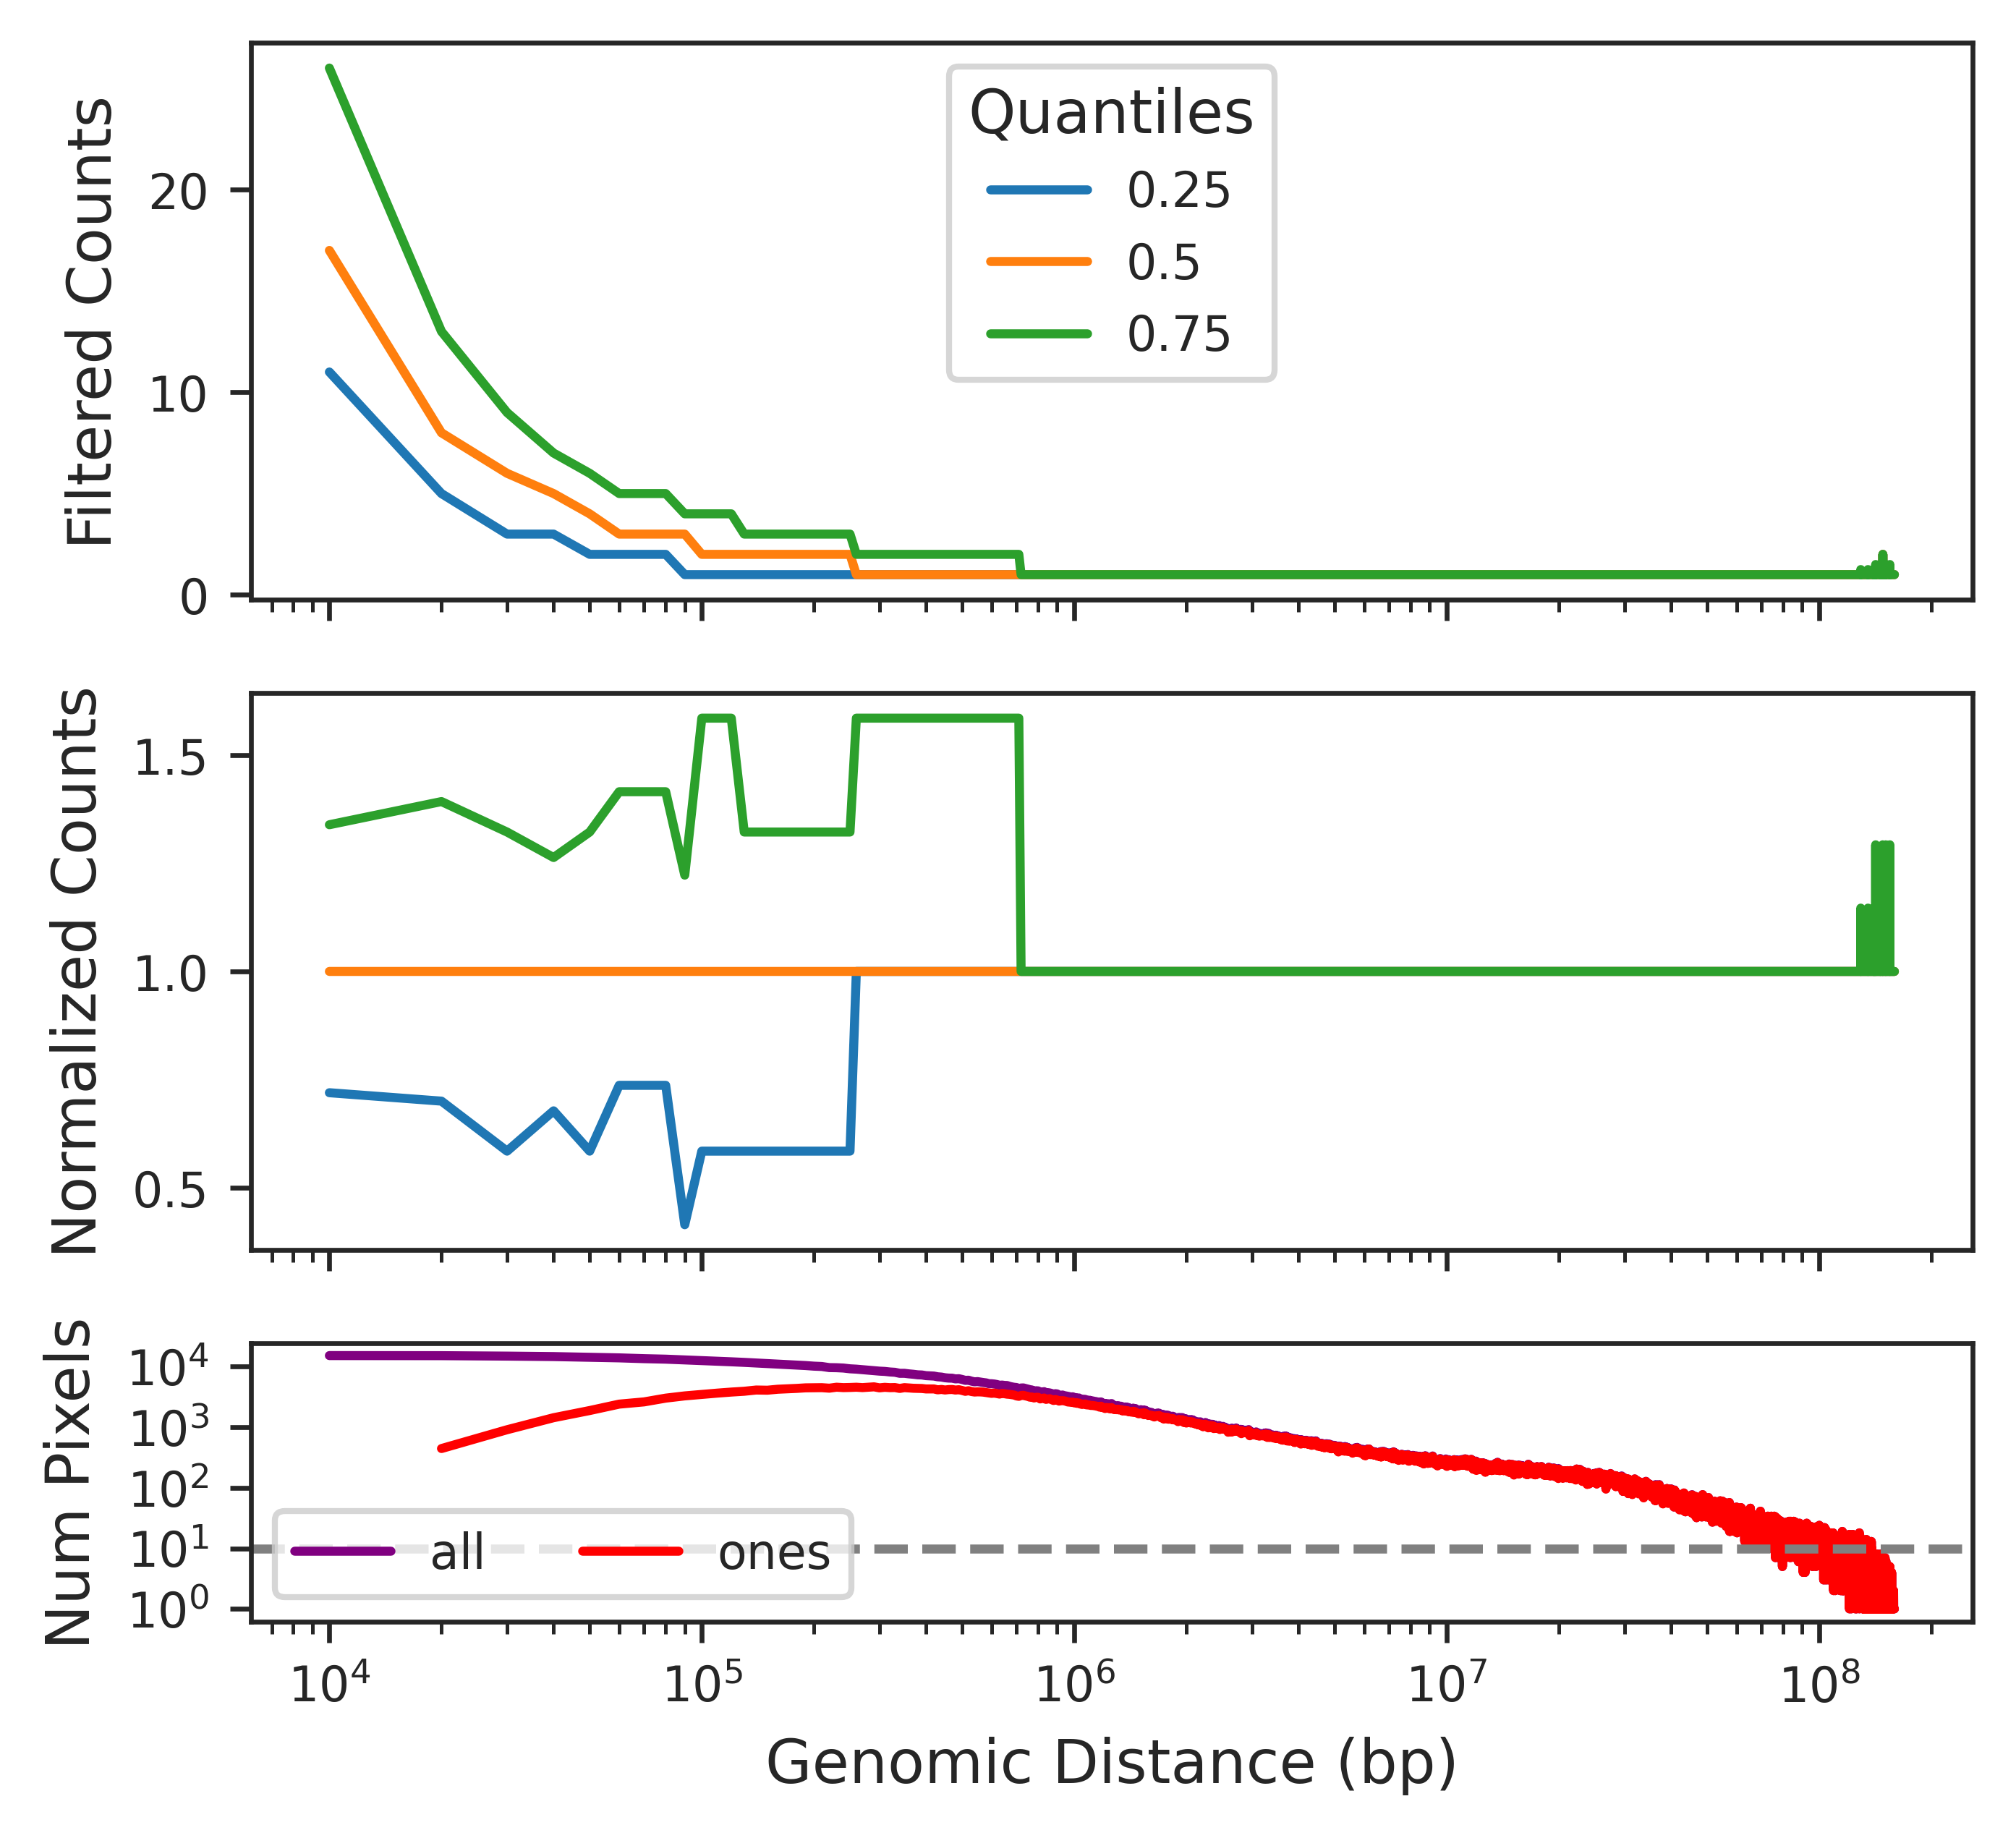
\includegraphics[width=0.5\textwidth]{normalization_rep1.png}
  \caption{\textbf{Replication data for figure \ref{fig:normstats}}. Comparison of the distribution of raw and normalized counts at each genomic distance for chromosome 7 of one replicate of IMR90 cells (4DNFIMU9T2QI), at 10 kb resolution, filtered using 200 Mb as genomic distance threshold.} 
\end{figure}

\begin{figure}[h]
  \centering
  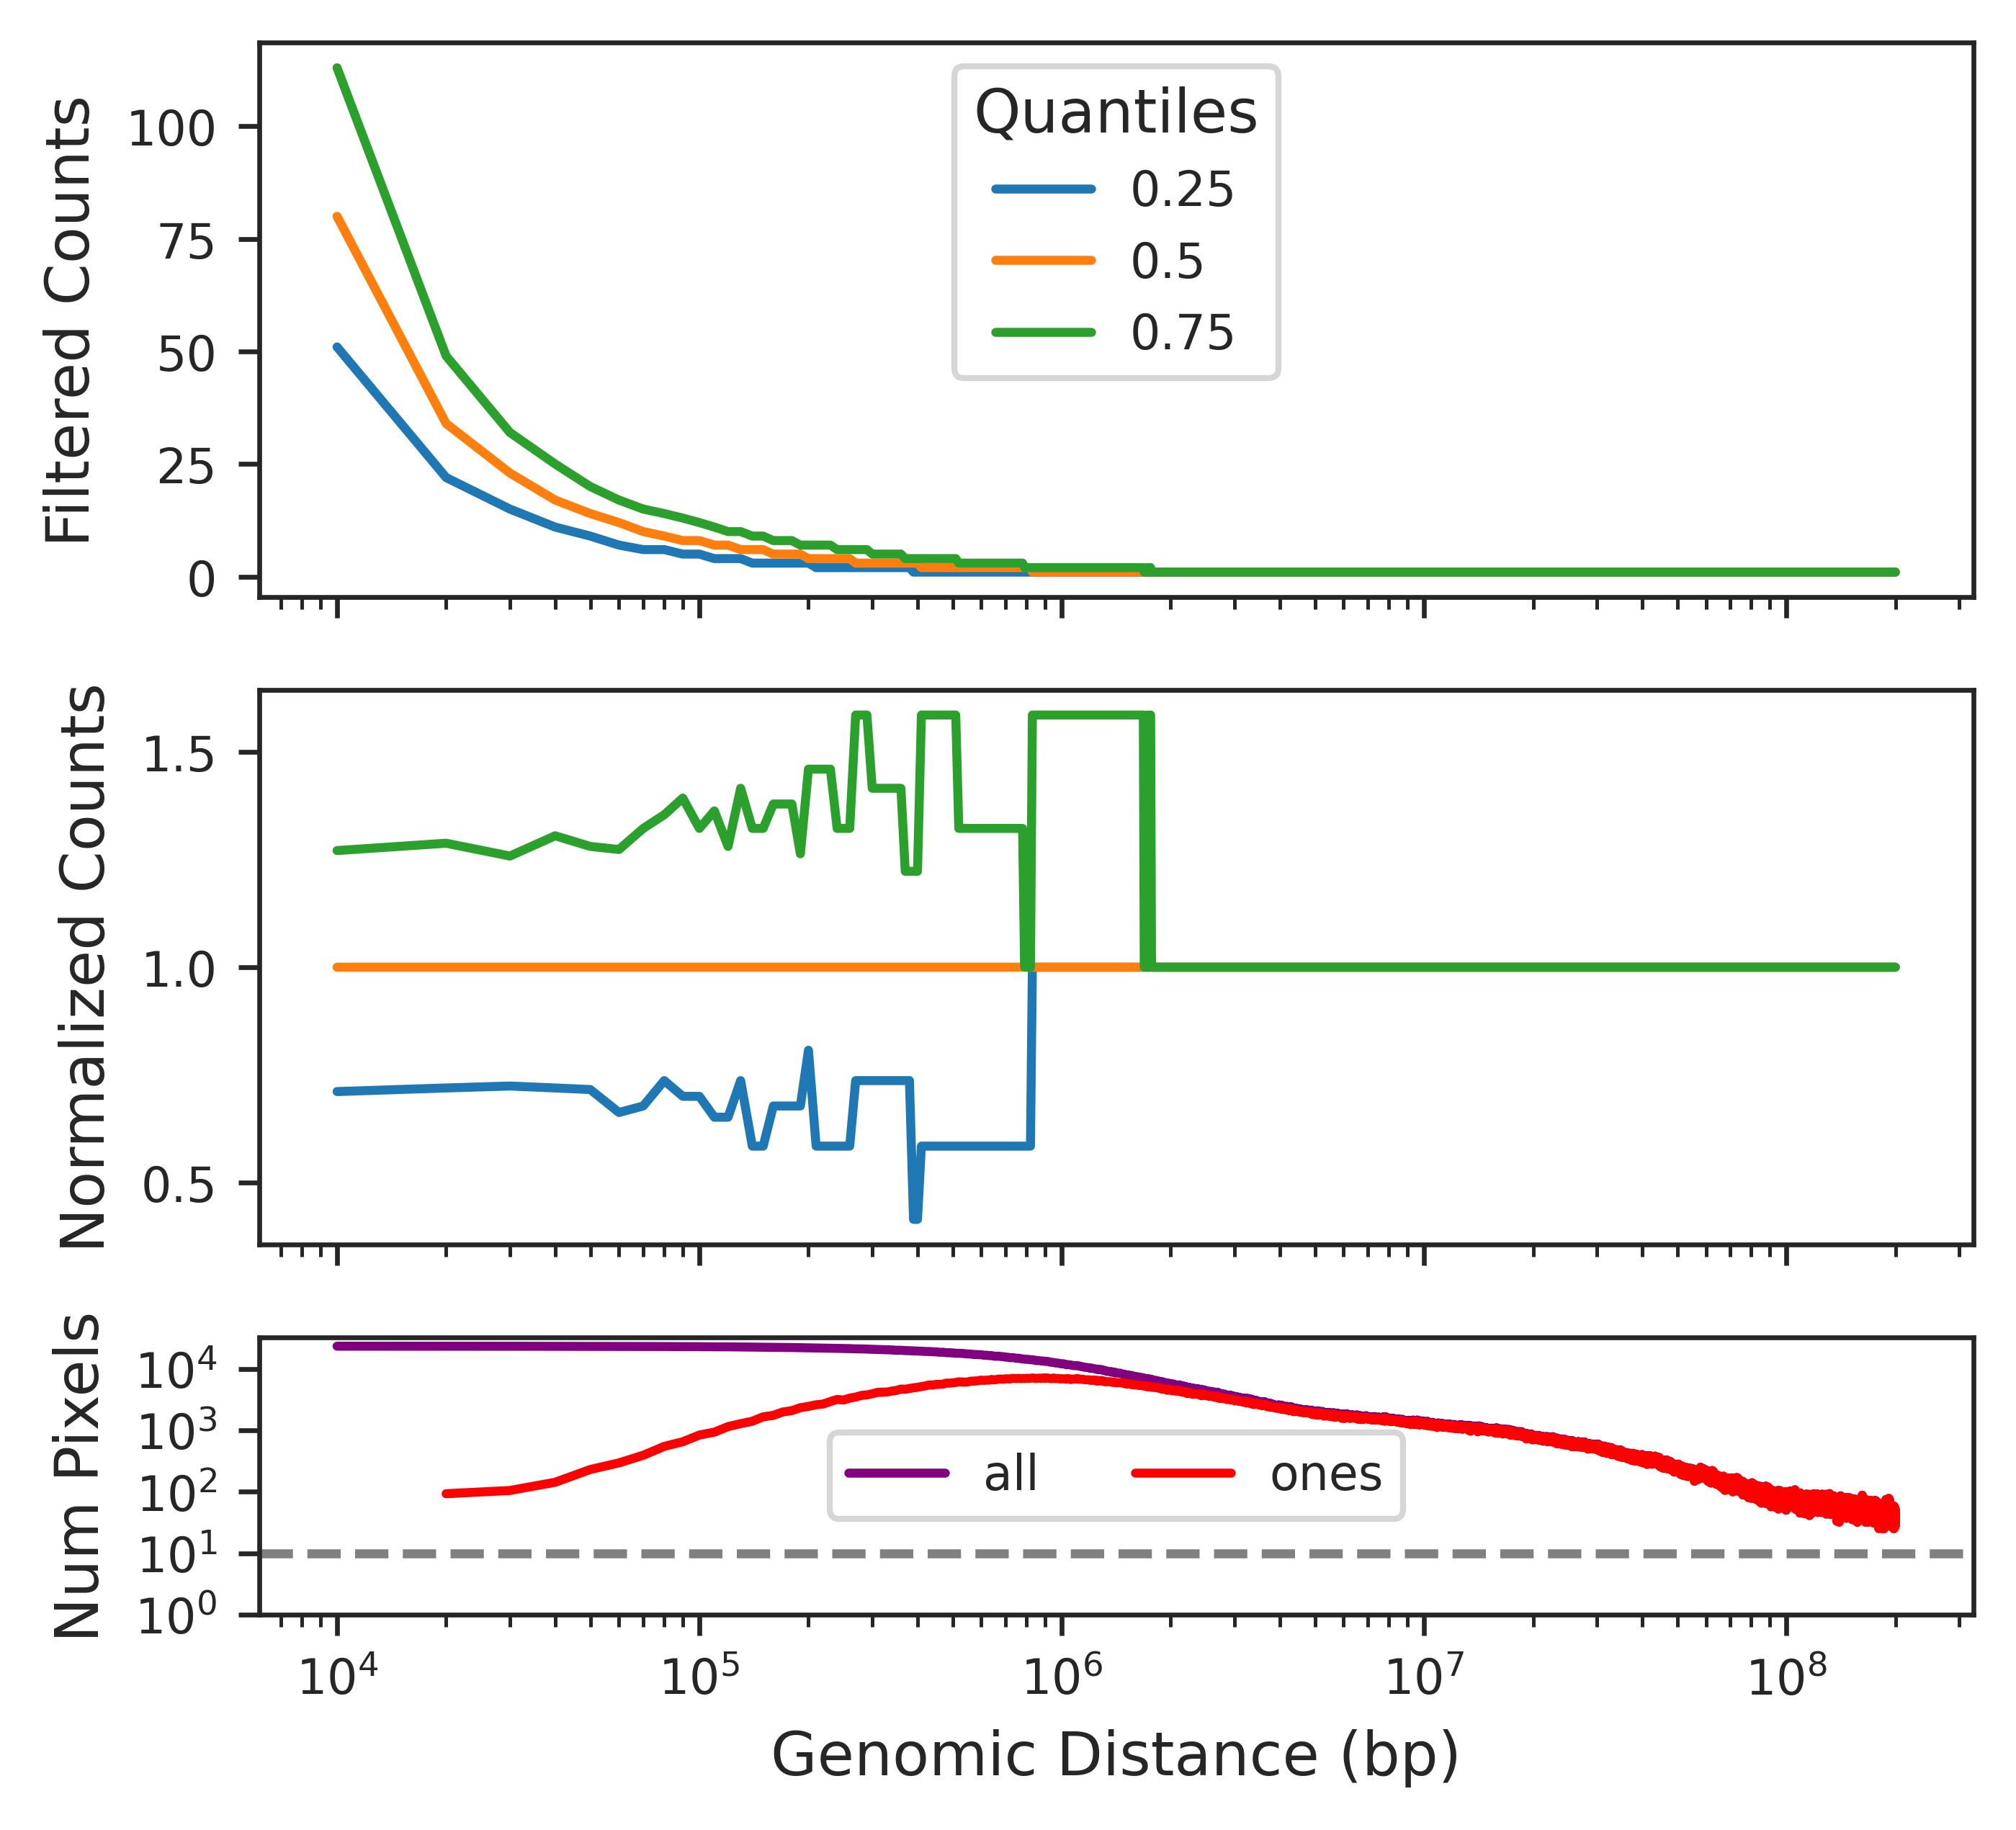
\includegraphics[width=0.5\textwidth]{normalization_rep2.png}
  \caption{\textbf{Replication data for figure \ref{fig:normstats}}. Comparison of the distribution of raw and normalized counts at each genomic distance for chromosome 2 of HMEC cells (4DNFIIFAUT24), at 10 kb resolution, filtered using 200 Mb as genomic distance threshold.} 
\end{figure}

\begin{figure}[h]
  \centering 
  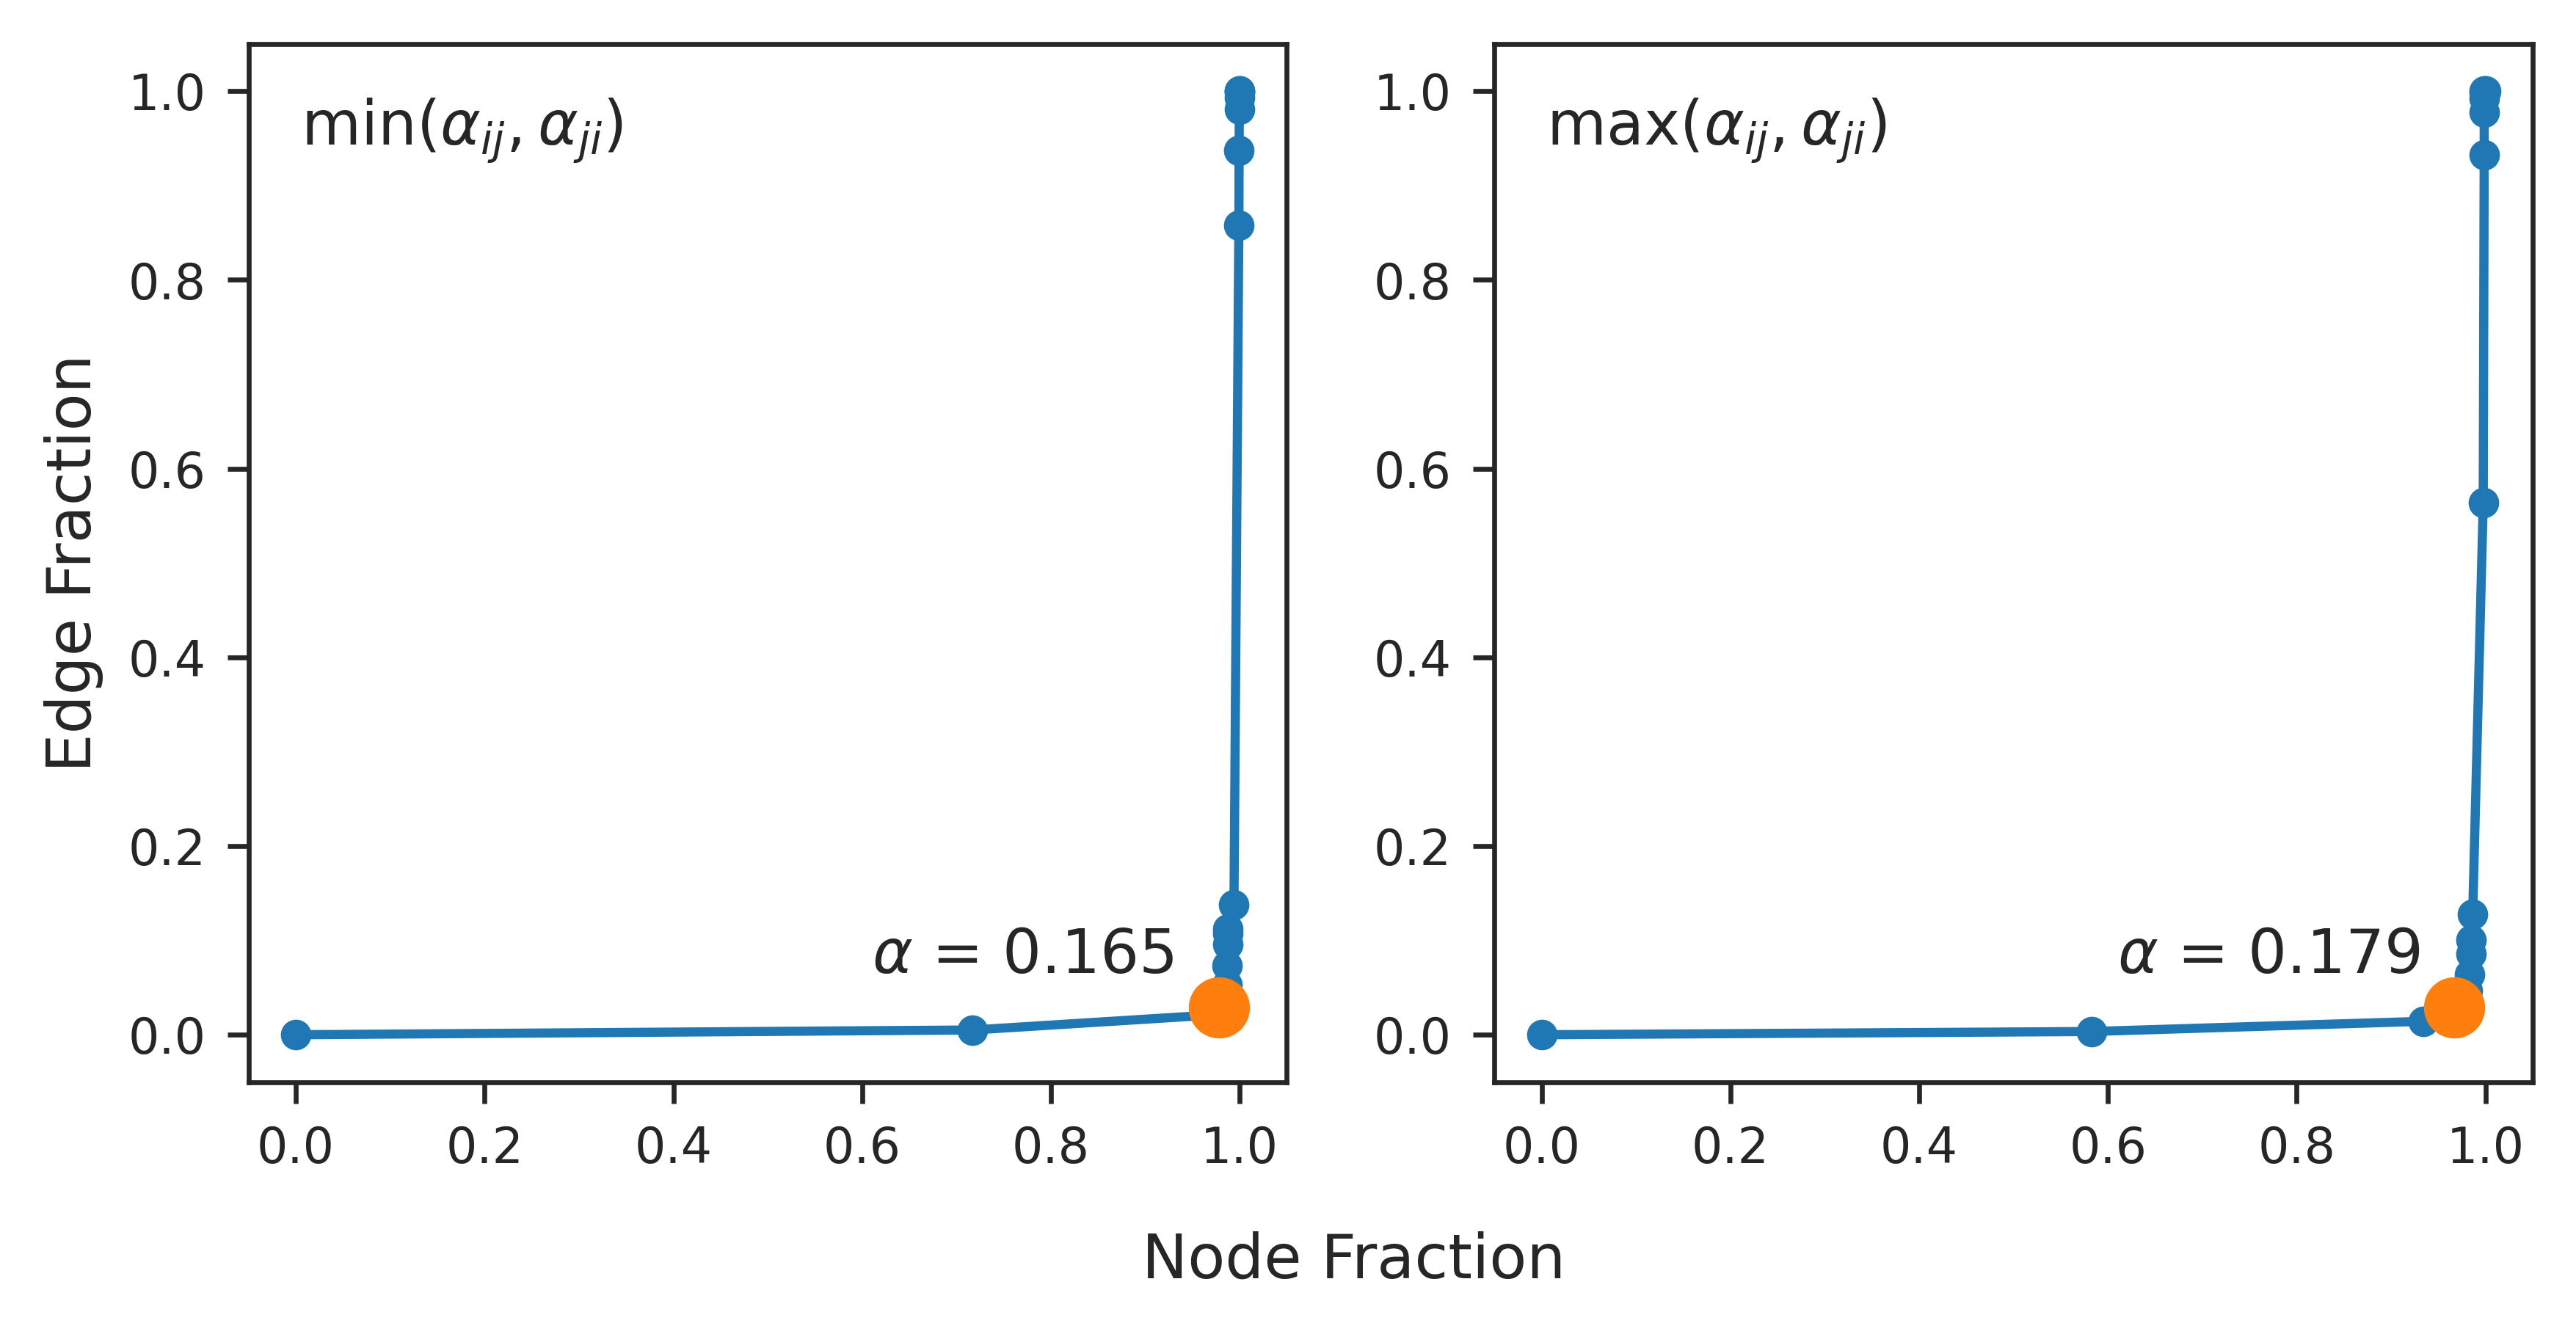
\includegraphics[width=0.7\textwidth]{alphas_rep1.png}
  \caption{\textbf{Replication data for figure \ref{fig:alphas}}. In the panels, sets of points tested to find the optimal alpha value for chromosome 1 of HMEC cells (4DNFIIFAUT24) at 10 kb resolution, processed using 200 Mb as distance threshold, 0 as quantile threshold.}
\end{figure}

\begin{figure}[h]
  \centering 
  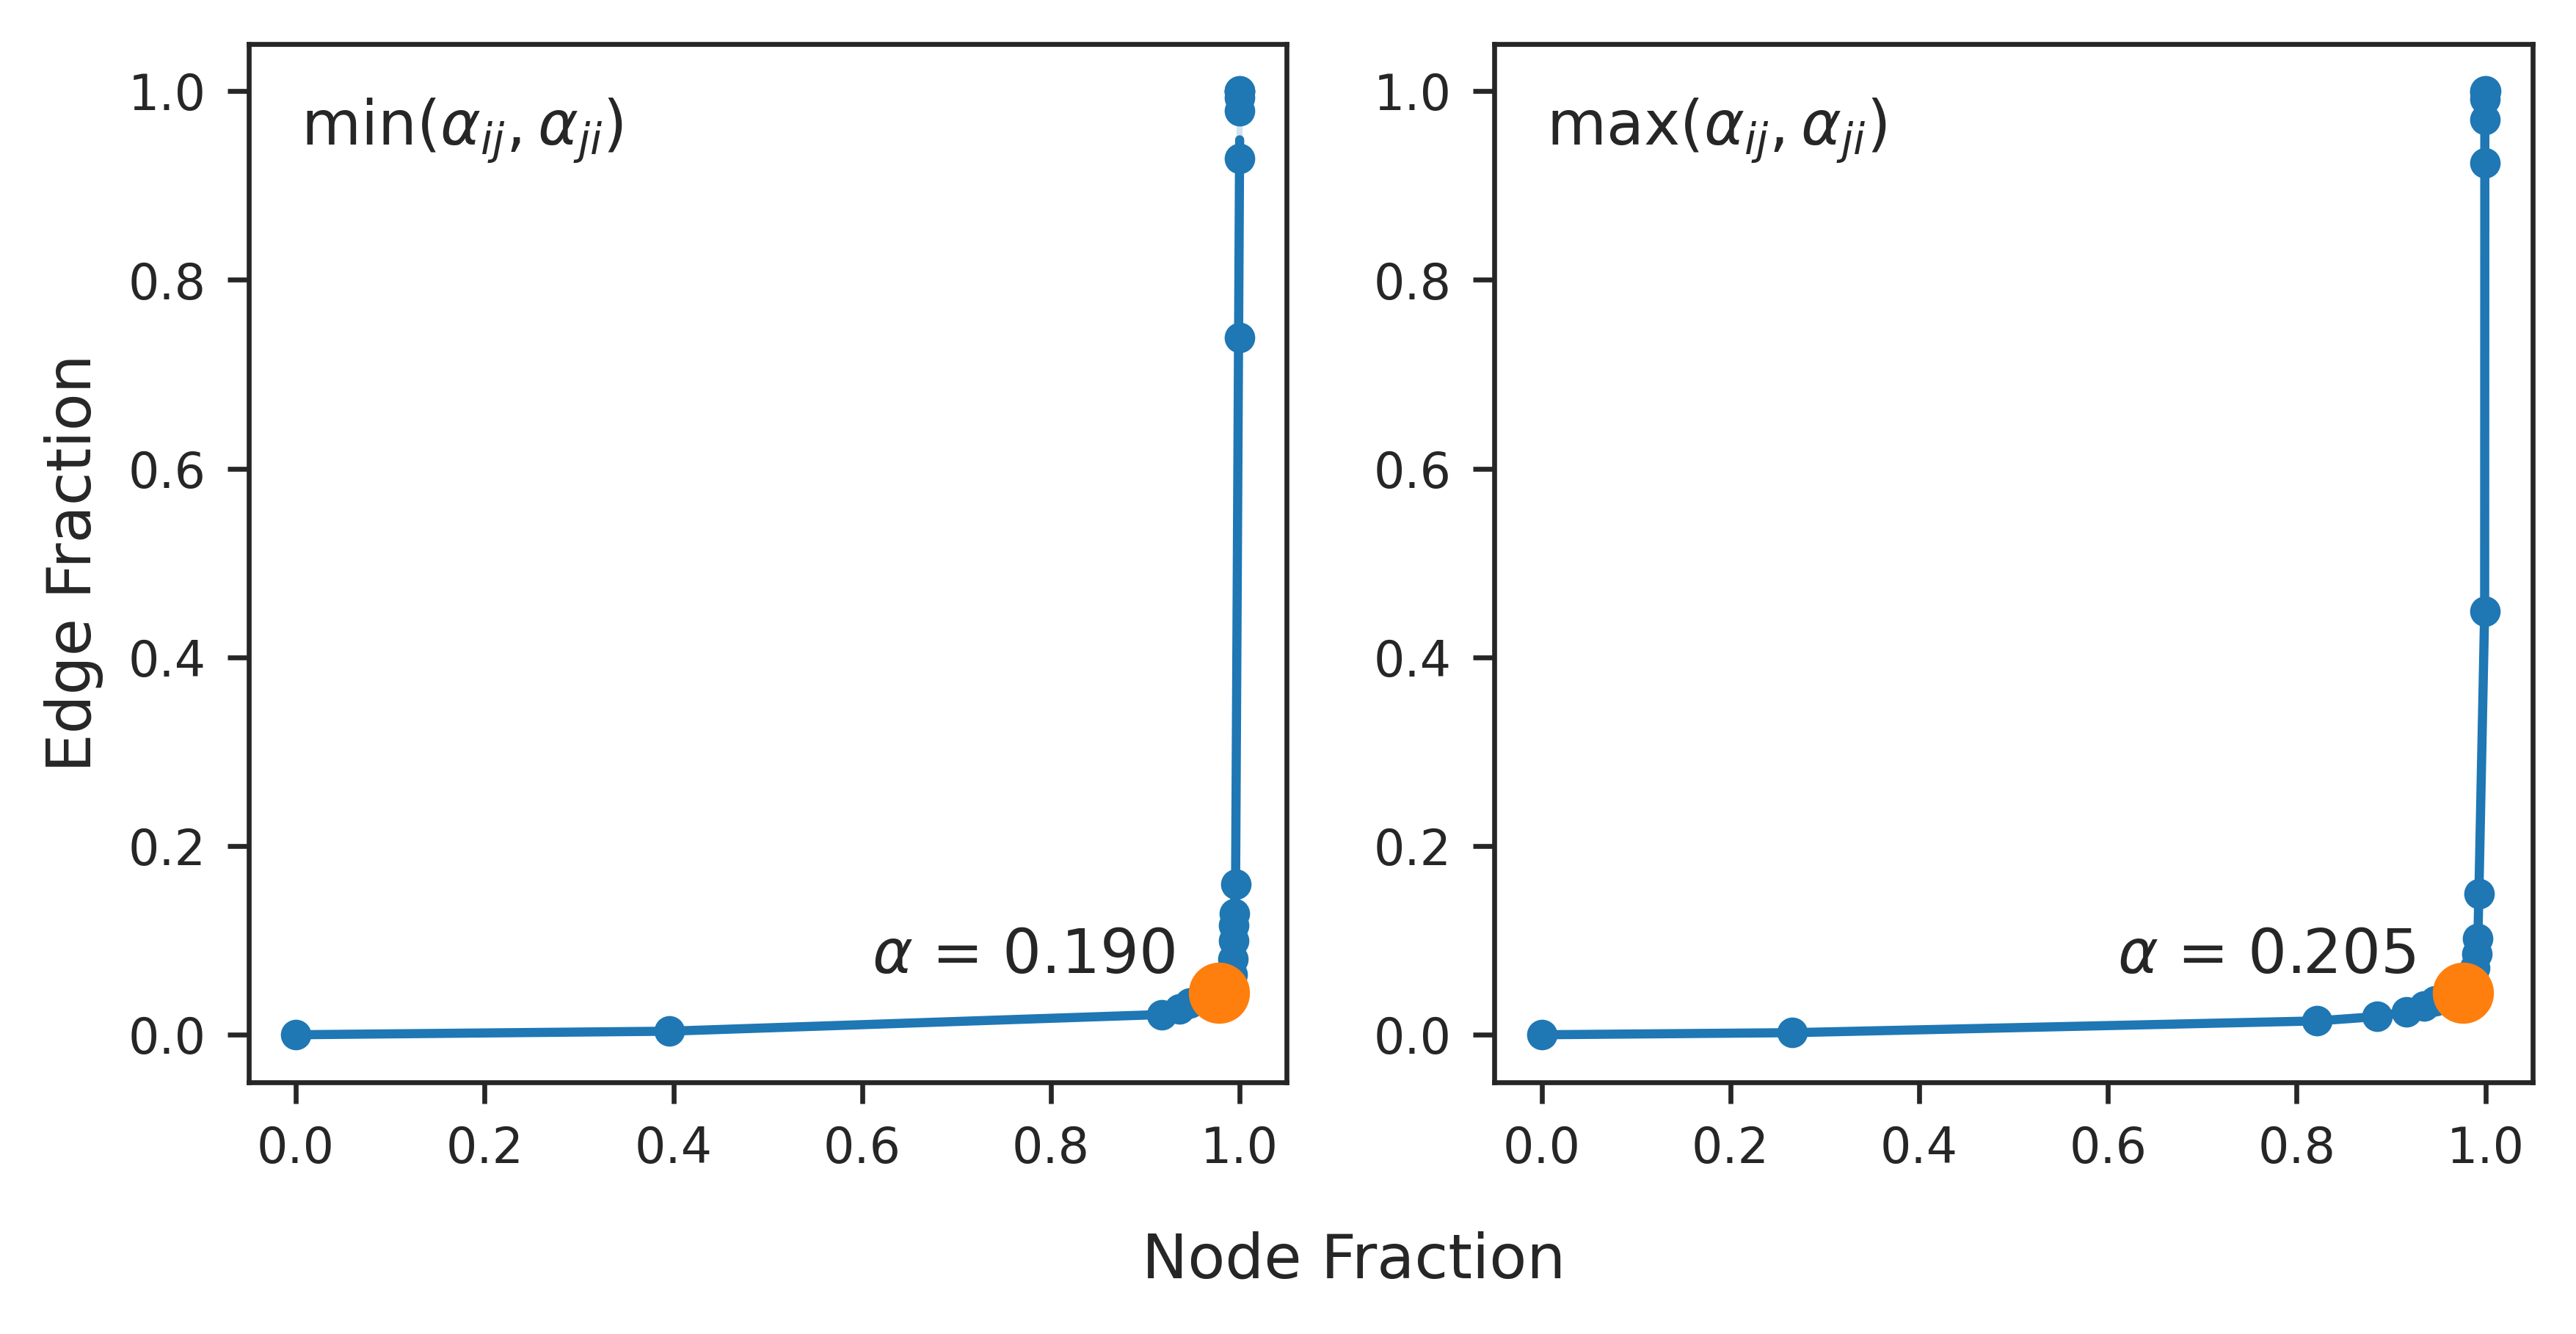
\includegraphics[width=0.7\textwidth]{alphas_rep3.png}
  \caption{\textbf{Replication data for figure \ref{fig:alphas}}. In the panels, sets of points tested to find the optimal alpha value for chromosome 19 of one replicate of IMR90 cells (4DNFIMU9T2QI) at 10 kb resolution, processed using 200 Mb as distance threshold, 0 as quantile threshold.}
\end{figure}

\begin{figure}[h]
  \centering 
  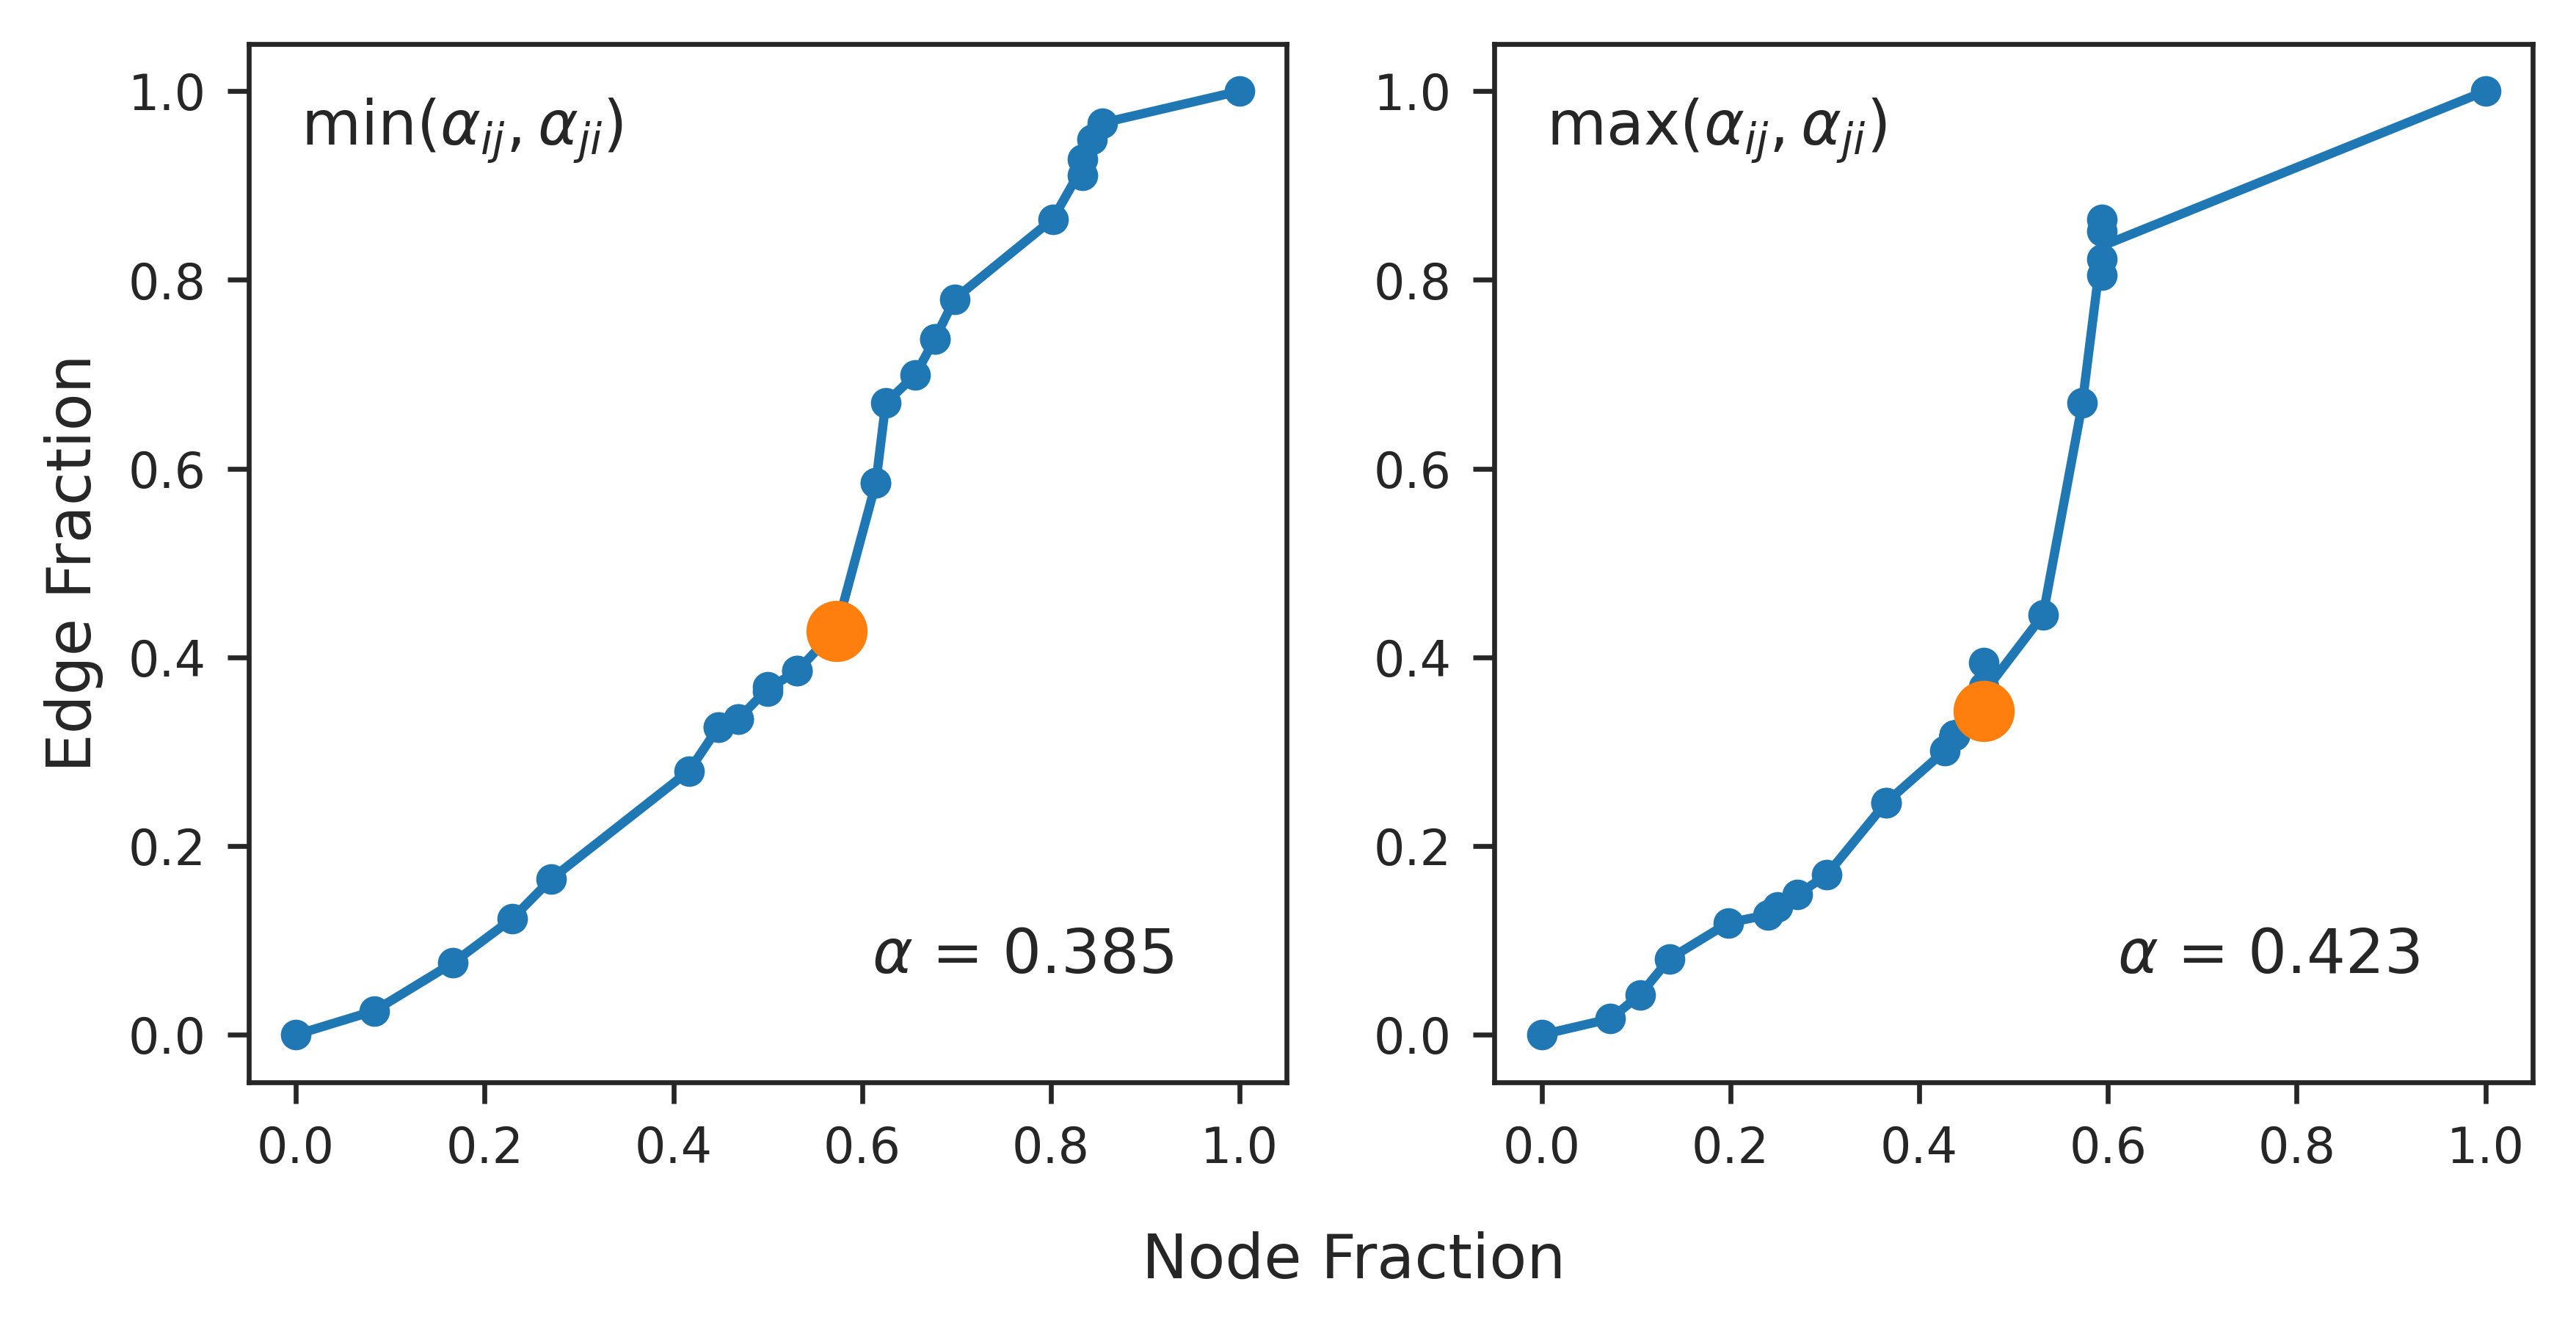
\includegraphics[width=0.7\textwidth]{alphas_rep2.png}
  \caption{\textbf{Replication data for figure \ref{fig:alphas}}. In the panels, sets of points tested to find the optimal alpha value for chromosome Y of one replicate of IMR90 cells (4DNFIMU9T2QI) at 10 kb resolution, processed using 200 Mb as distance threshold, 0 as quantile threshold. Reported to show the instability of the procedure on chromosome Y.}
\end{figure}

\begin{figure}[h]
  \centering 
  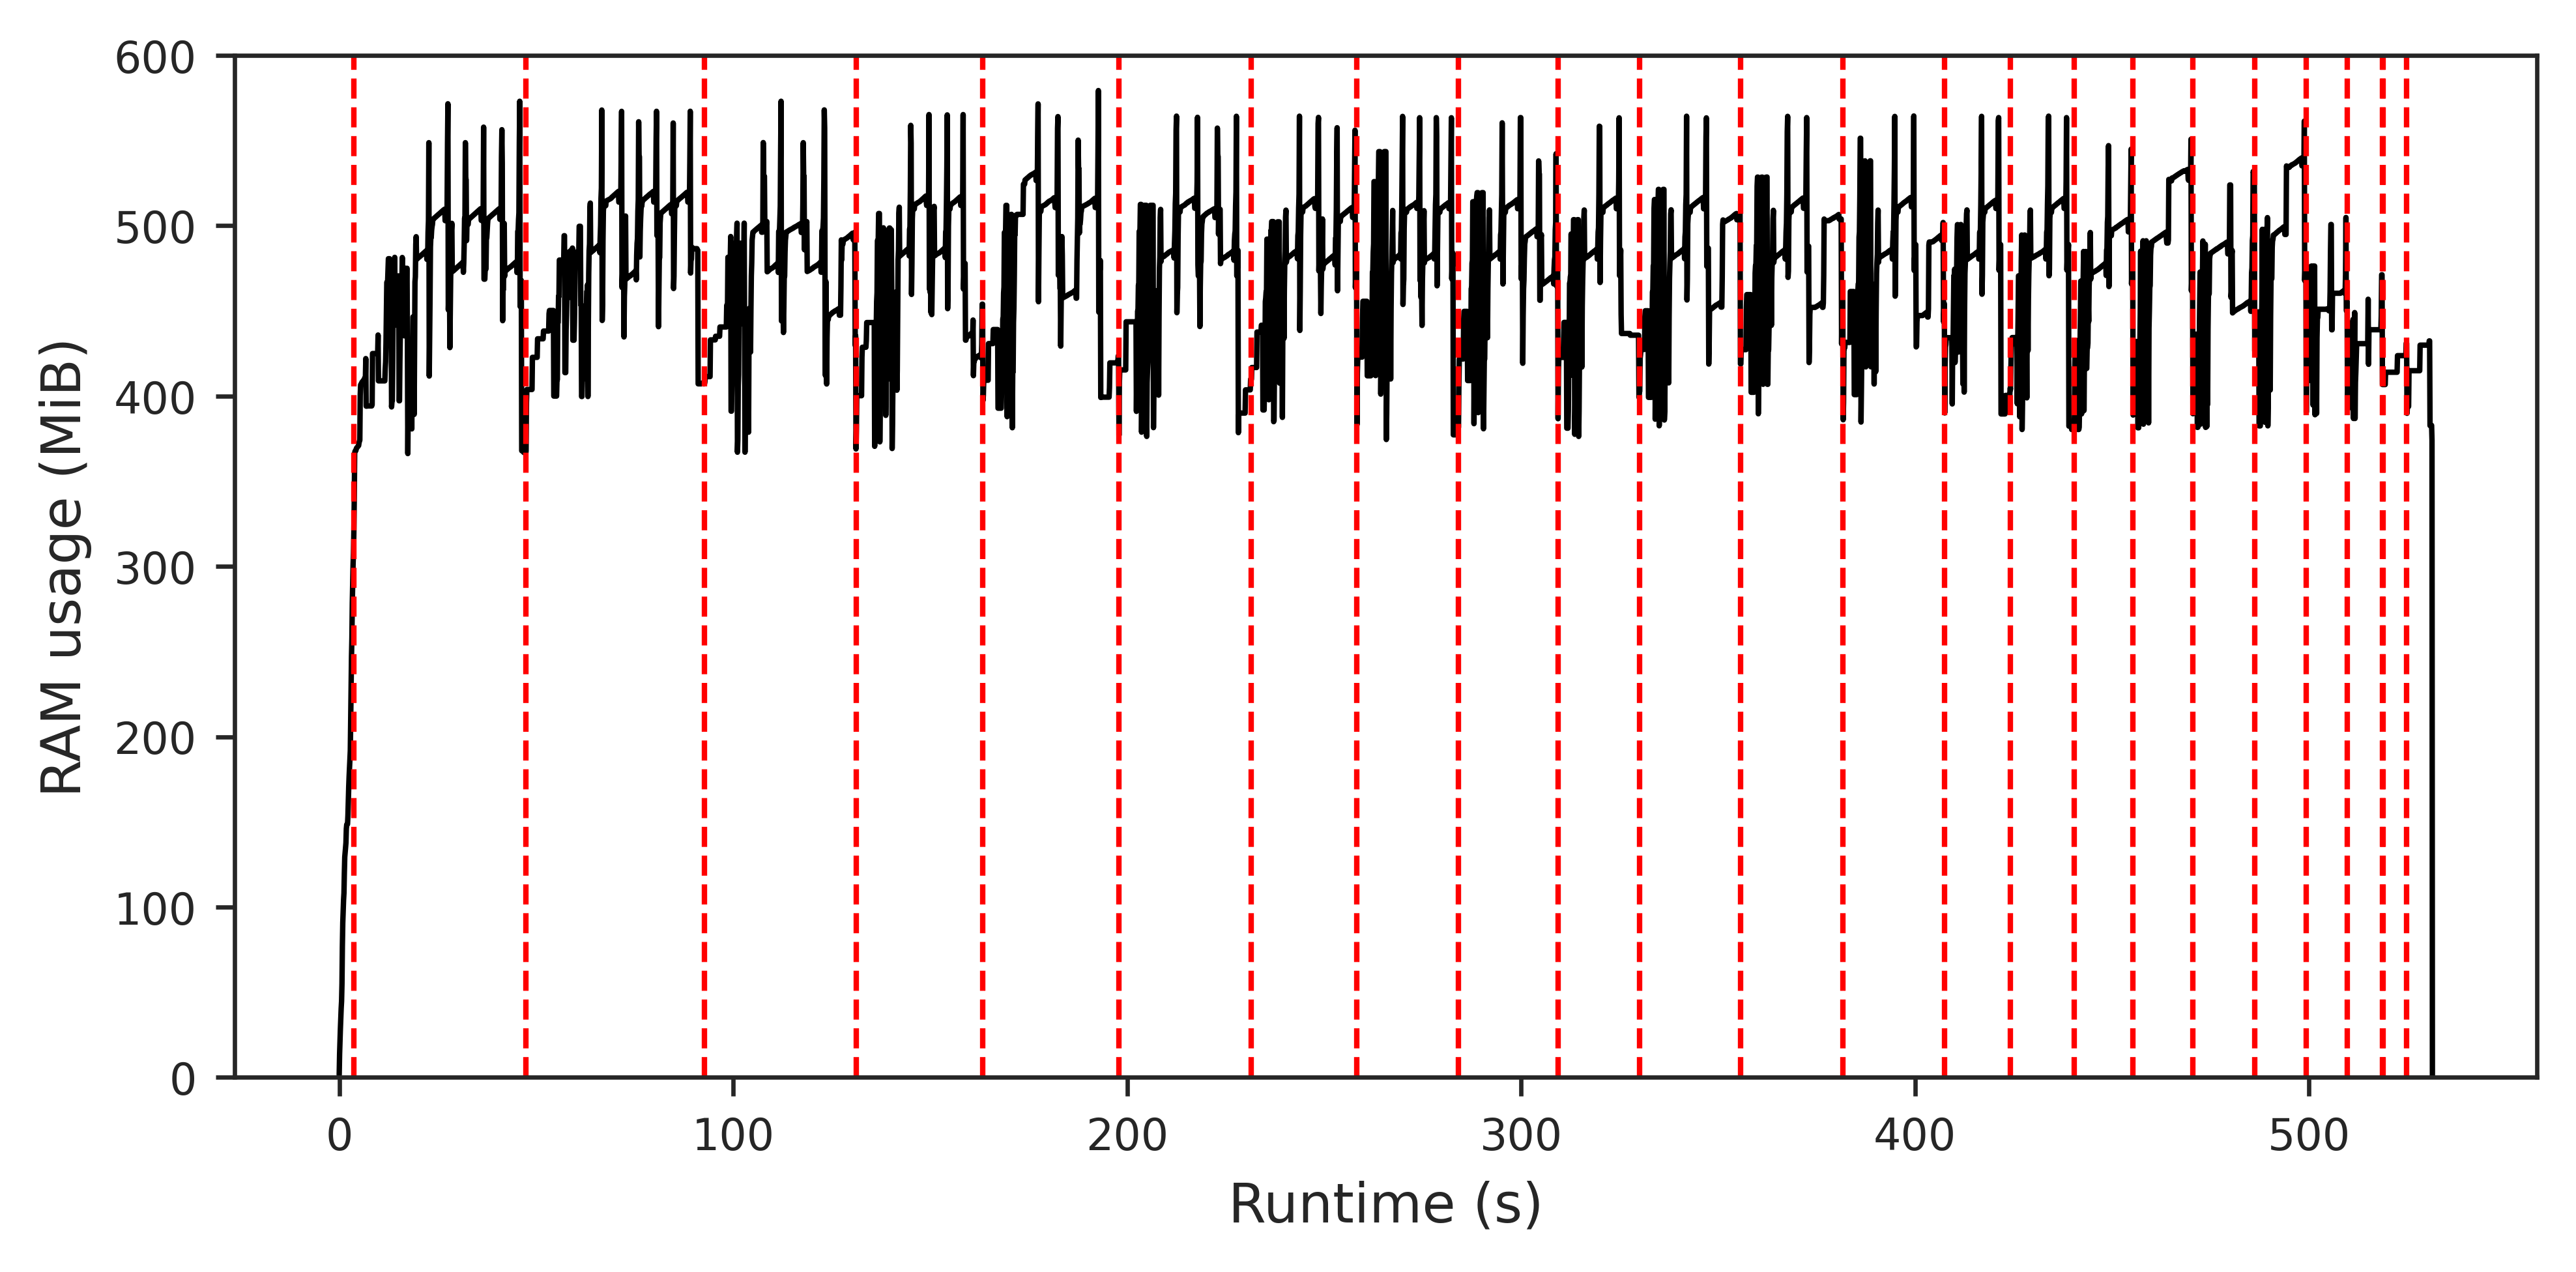
\includegraphics[width=1\textwidth]{memory_benchmark.png}
  \caption{\textbf{Replication data for figure \ref{fig:memorybenchmark}}. Plot of Random Access Memory usage during the preprocessing procedure. Runtime is expressed in seconds, while memory usage is expressed in MebiBytes (1 MiB = $2^{20}$ bytes). The area included between two red dashed lines corresponds to the sparsification scores computation for a chromosome. In the figure, the RAM usage overtime for HMEC cells (4DNFIIFAUT24) at 10 kb resolution, processed using 100 Mb as distance threshold, 0.01 as quantile threshold, is shown.}
\end{figure}